\documentclass[svgnames,11pt]{beamer}
\input{/home/tof/Documents/Cozy/latex-include/preambule_commun.tex}
\input{/home/tof/Documents/Cozy/latex-include/preambule_beamer.tex}
%\usepackage{pgfpages} \setbeameroption{show notes on second screen=left}
\author[]{Christophe Viroulaud}
\title{Géoportail}
\date{\framebox{\textbf{Loc 02}}}
%\logo{}
\institute{Seconde - SNT}
\usepackage{multimedia}
\begin{document}
\begin{frame}
    \titlepage
        \note[item]{\fcolorbox{black}{red}{{\LARGE geoportail-annexe.zip}}}
        \note[item]{\fcolorbox{black}{red}{{\LARGE section 1 au tableau}}}
        \note[item]{\fcolorbox{black}{red}{{\LARGE section 2 en autonomie}}}
\end{frame}
\begin{frame}
    \frametitle{}

    L'\emph{Institut Géographique National (IGN)} est un établissement public à caractère administratif ayant pour mission d'assurer la production, l'entretien et la diffusion de l'information géographique de référence en France.
    \begin{center}
        \centering
        
\includegraphics[width=4cm]{ressources/ign.png}
    \end{center}
    \note{intégration de l'inventaire forestier national le 1er janvier 2012, mais conserve sigle \textbf{IGN}}
\end{frame}
\begin{frame}
    \frametitle{}
    L'IGN fournit un site web: \emph{Géoportail} qui propose de nombreuses informations, fonds de cartes dessinés par des cartographes.
    \begin{center}
        \framebox{Quelles sont les fonctionnalités du Géoportail?}
    \end{center}

\end{frame}
\section{L'IGN}
\subsection{Mission}
\begin{frame}
    \frametitle{Mission}

    \begin{center}
        {\Large Observer - Mesurer - Décrire le territoire}
        \begin{center}
            \centering
            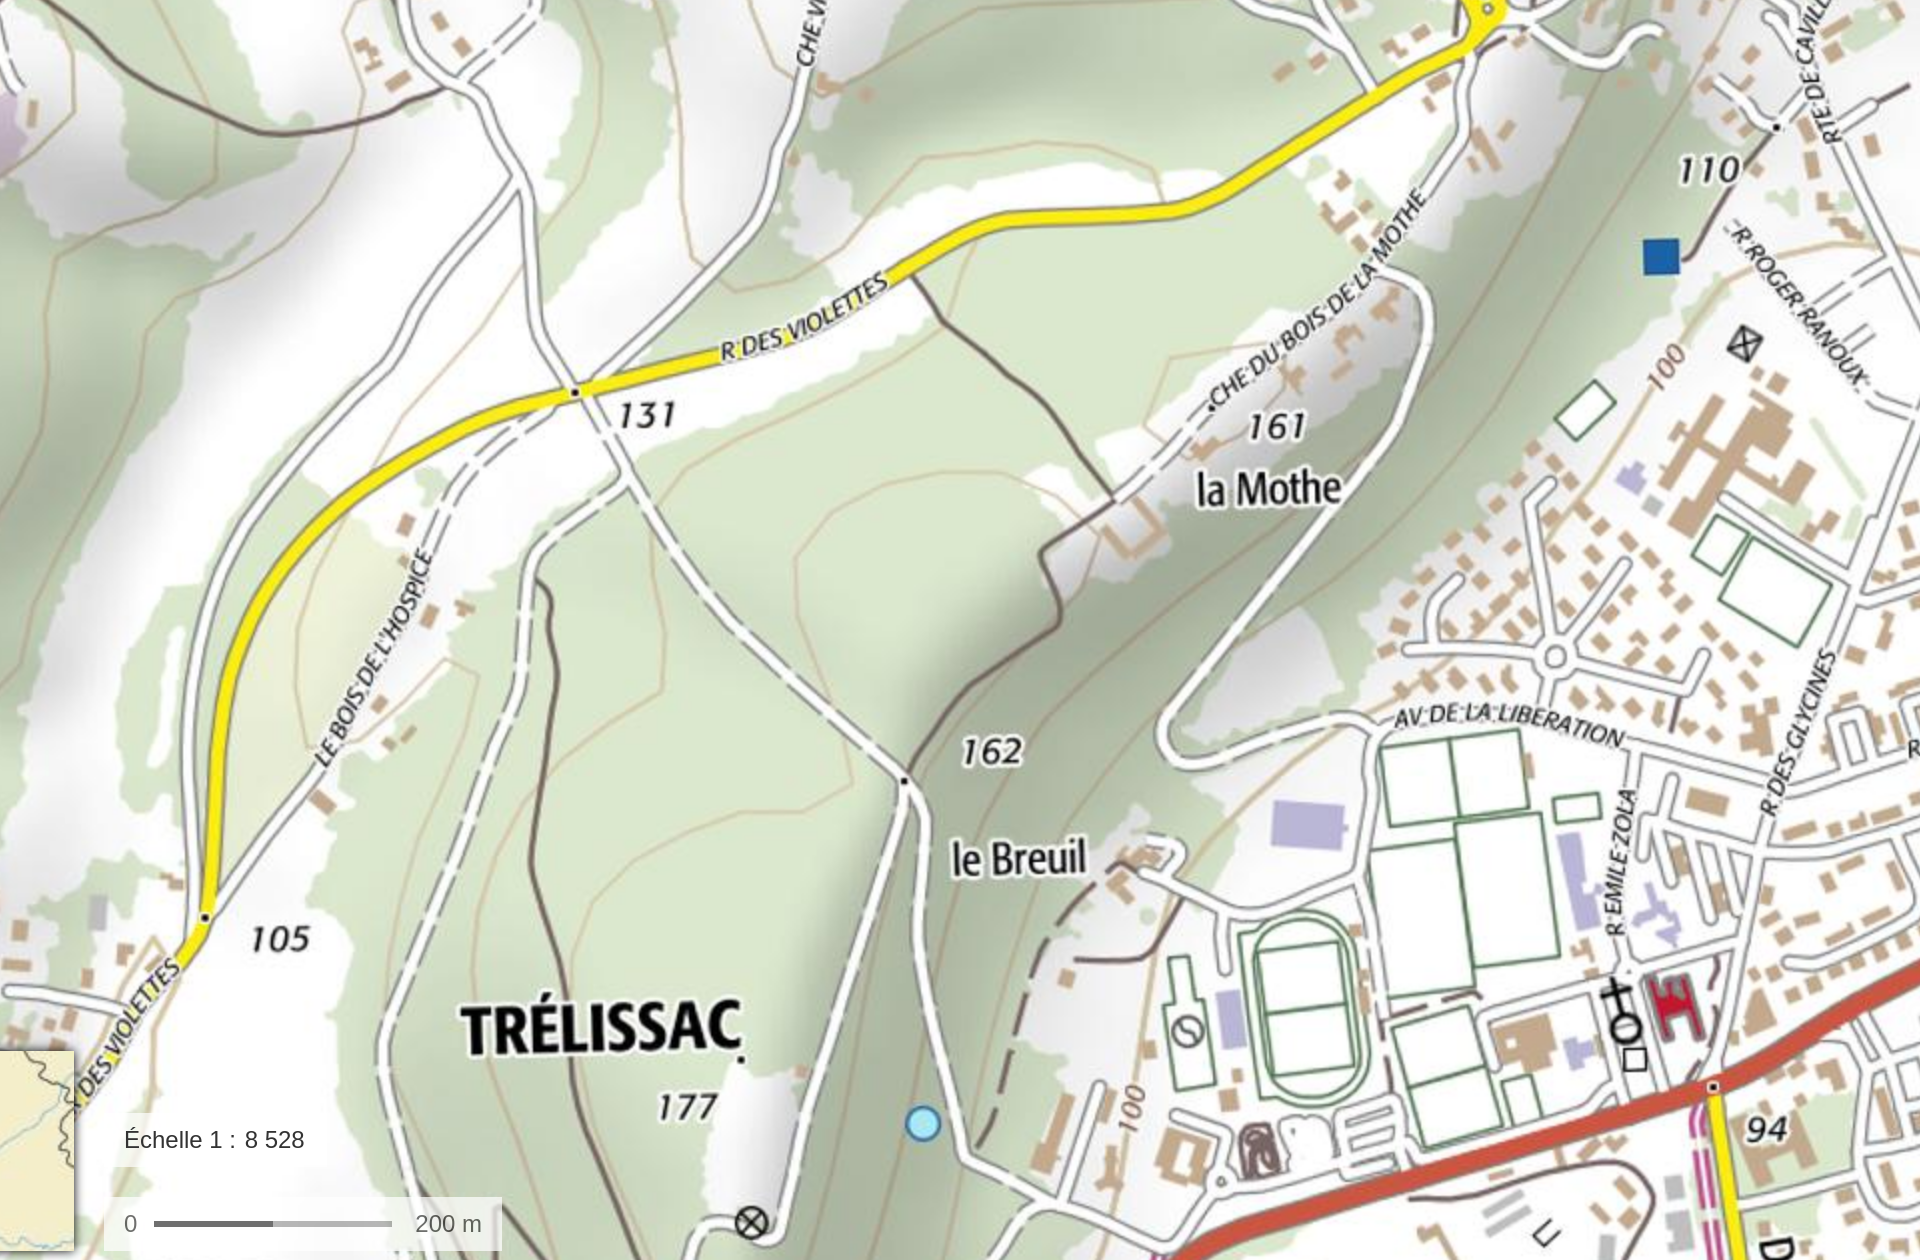
\includegraphics[width=9cm]{ressources/mission-ign.png}
            \captionof{figure}{Carte topographique}
            \label{IMG}
        \end{center}
    \end{center}
\end{frame}
\begin{frame}
    \frametitle{}

    \begin{itemize}
        \item Garantir la disponibilité des données géolocalisées et notamment des données souveraines pour l'État.
        \item Favoriser l’appropriation et l’usage de la donnée géographique.
        \item Maintenir un niveau de compétences élevé dans le domaine de l'information géographique.

    \end{itemize}

\end{frame}
\begin{frame}
    \frametitle{À quoi servent les geodata?}
     
\begin{center}
    \href{ressources/geodata.mp4}{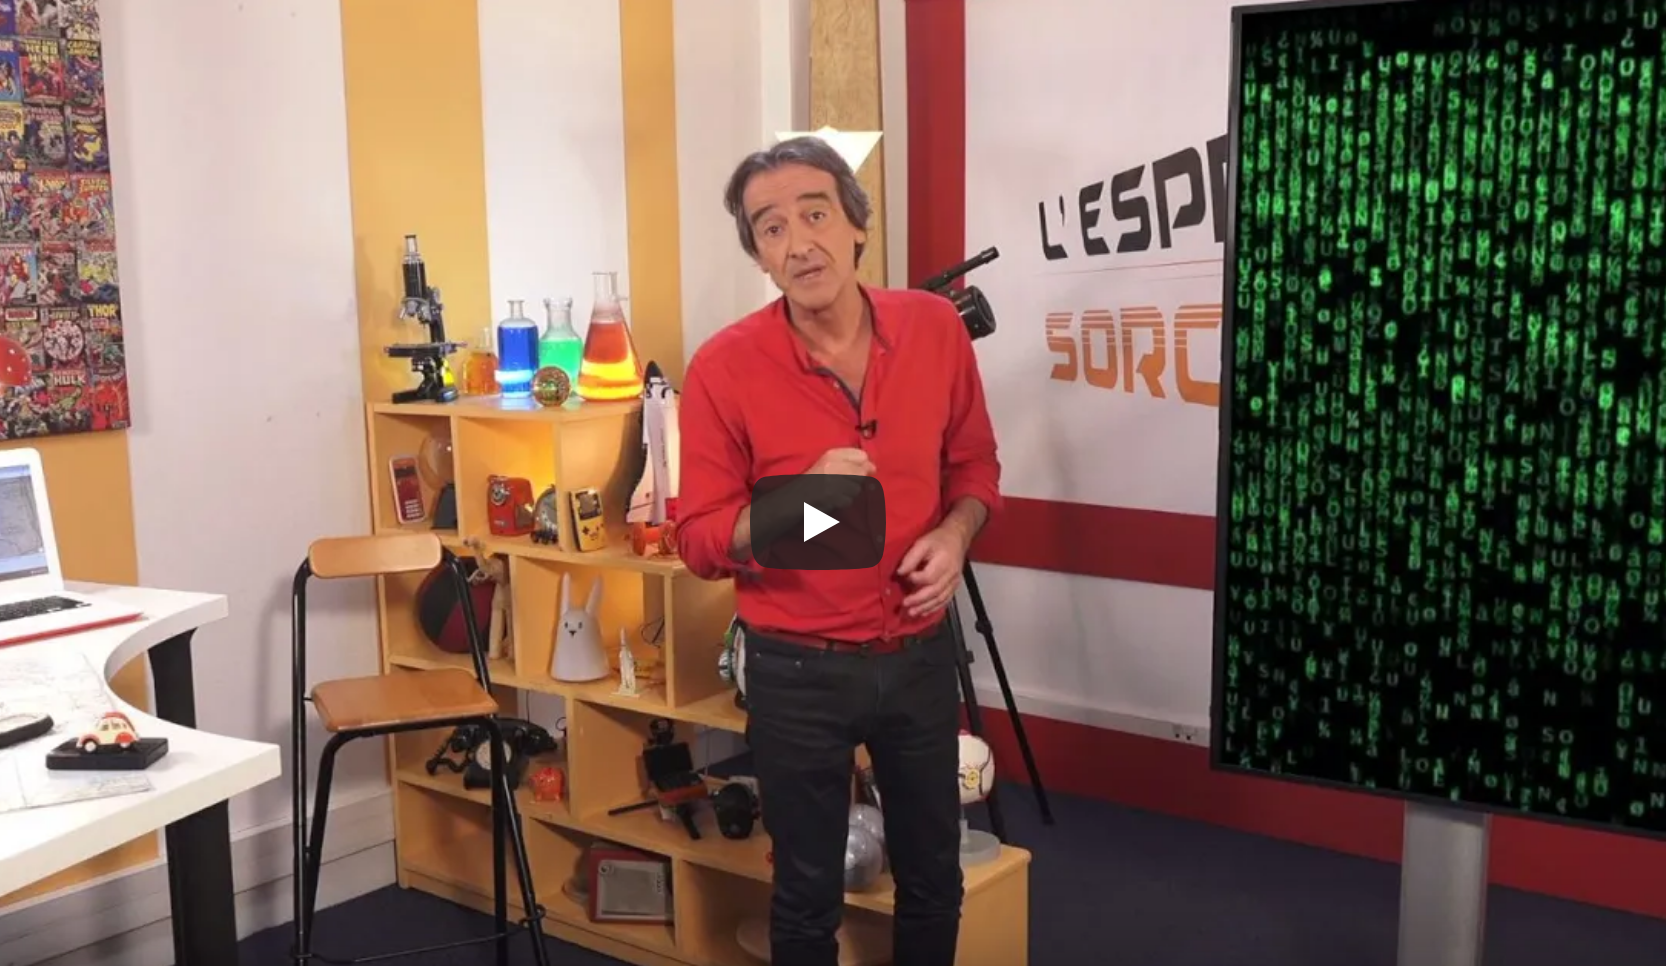
\includegraphics[width=8cm]{ressources/geodata.png}}

\end{center}
\end{frame}
\begin{frame}
    \frametitle{}

    \begin{activite}
    \begin{enumerate}
        \item Quelle est l'origine du mot \emph{géodata}?
        \item Quelles informations peut contenir une géodata?
        \item Qu'est-ce qu'un \emph{géomaticien}?
        \item Citer au moins trois applications des géodatas.
        \item Se rendre sur \url{https://tinyurl.com/igncotes}.
        \item Passer la souris sur les différentes photos. Quelle information obtient-on?
        \item Que peut-on dire de l'évolution des côtes françaises?
    \end{enumerate}
    \end{activite}
\note[item]{correction en commun}
\note[item]{frontière France/Italie qui varie en fonction mouvements plaques $\leftarrow$ IGN surveille et redéfinit frontière}
\end{frame}
\subsection{Moyens technologiques}
\begin{frame}
    \frametitle{Moyens technologiques}
\begin{itemize}
    \item \textbf{Géoplateforme}: mutualisation des données entre l'IGN et ses partenaires,
    \item \textbf{Lidar HD}: relevé laser de grande précision
    \item \dots
\end{itemize}
    

\end{frame}
\begin{frame}
    \frametitle{}

    \begin{center}
        \centering
        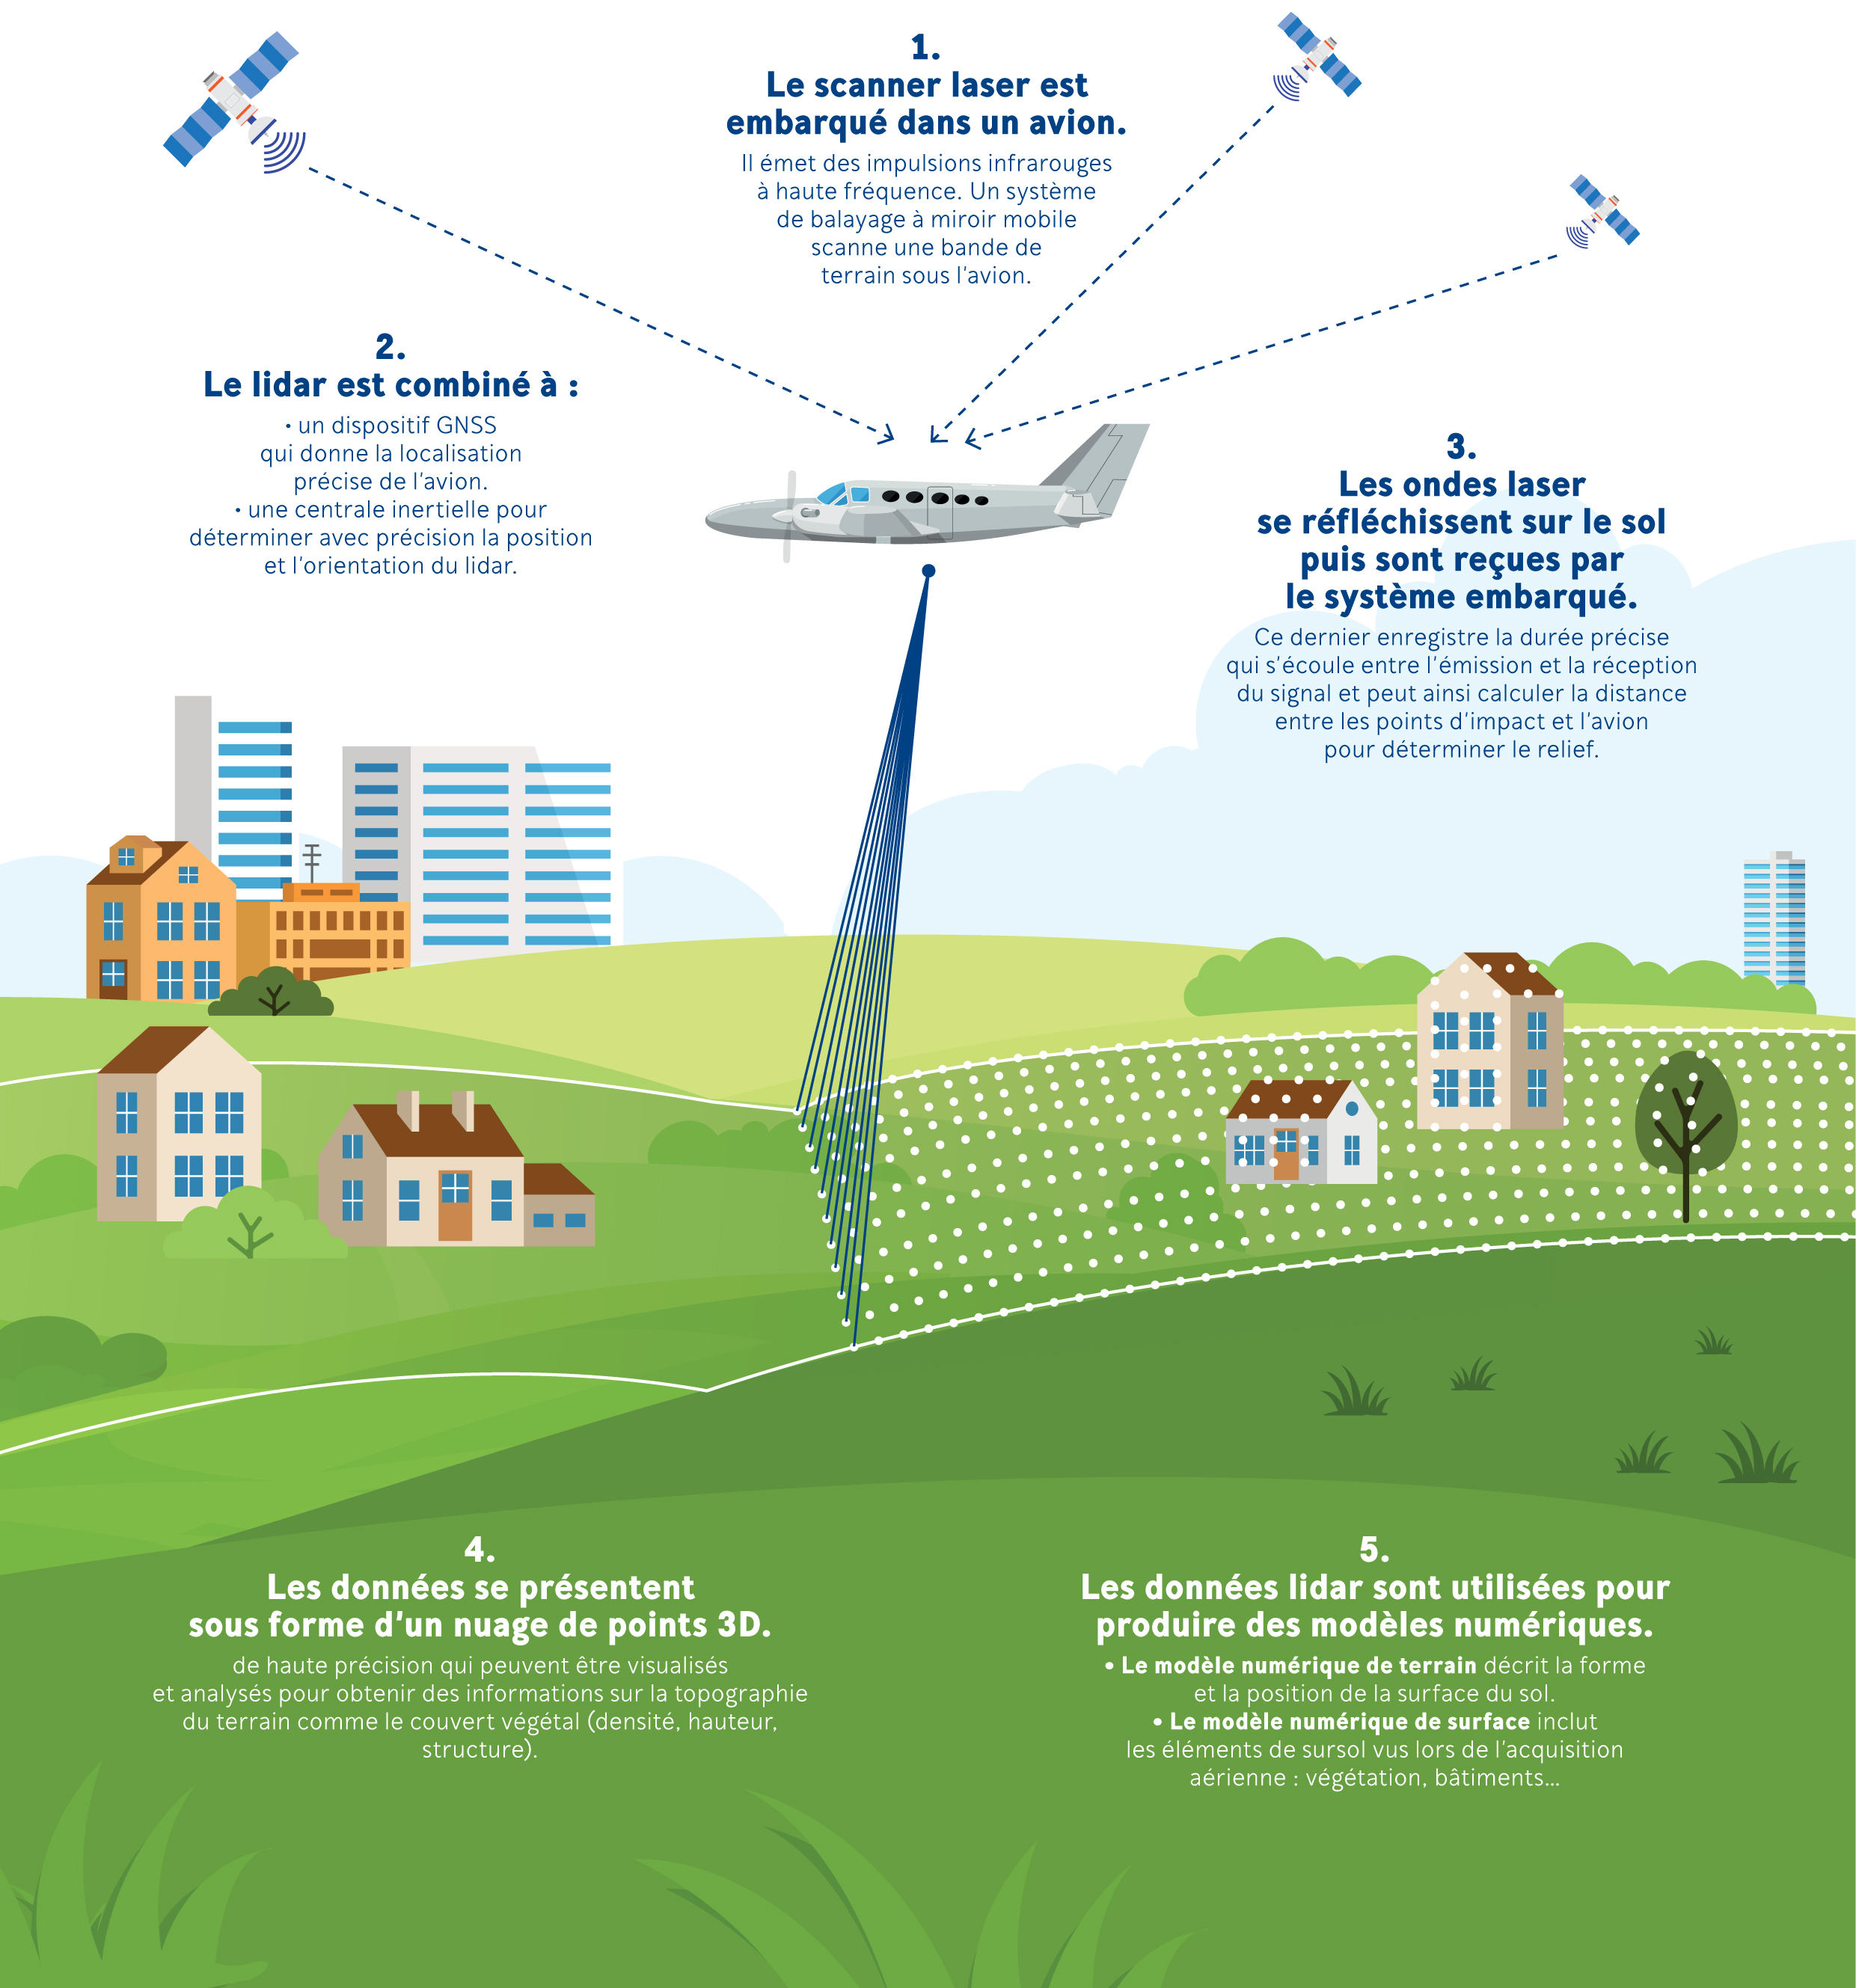
\includegraphics[width=8cm]{ressources/lidar.jpg}
        \end{center}
\note{tellement précis qu'on peut utiliser pour déterminer essence des arbres}
\end{frame}
\section{Géoportail}
\begin{frame}
    \frametitle{Géoportail}
C'est le site web qui permet d'accéder aux données fournies par l'IGN.
    \begin{center}
    \centering
    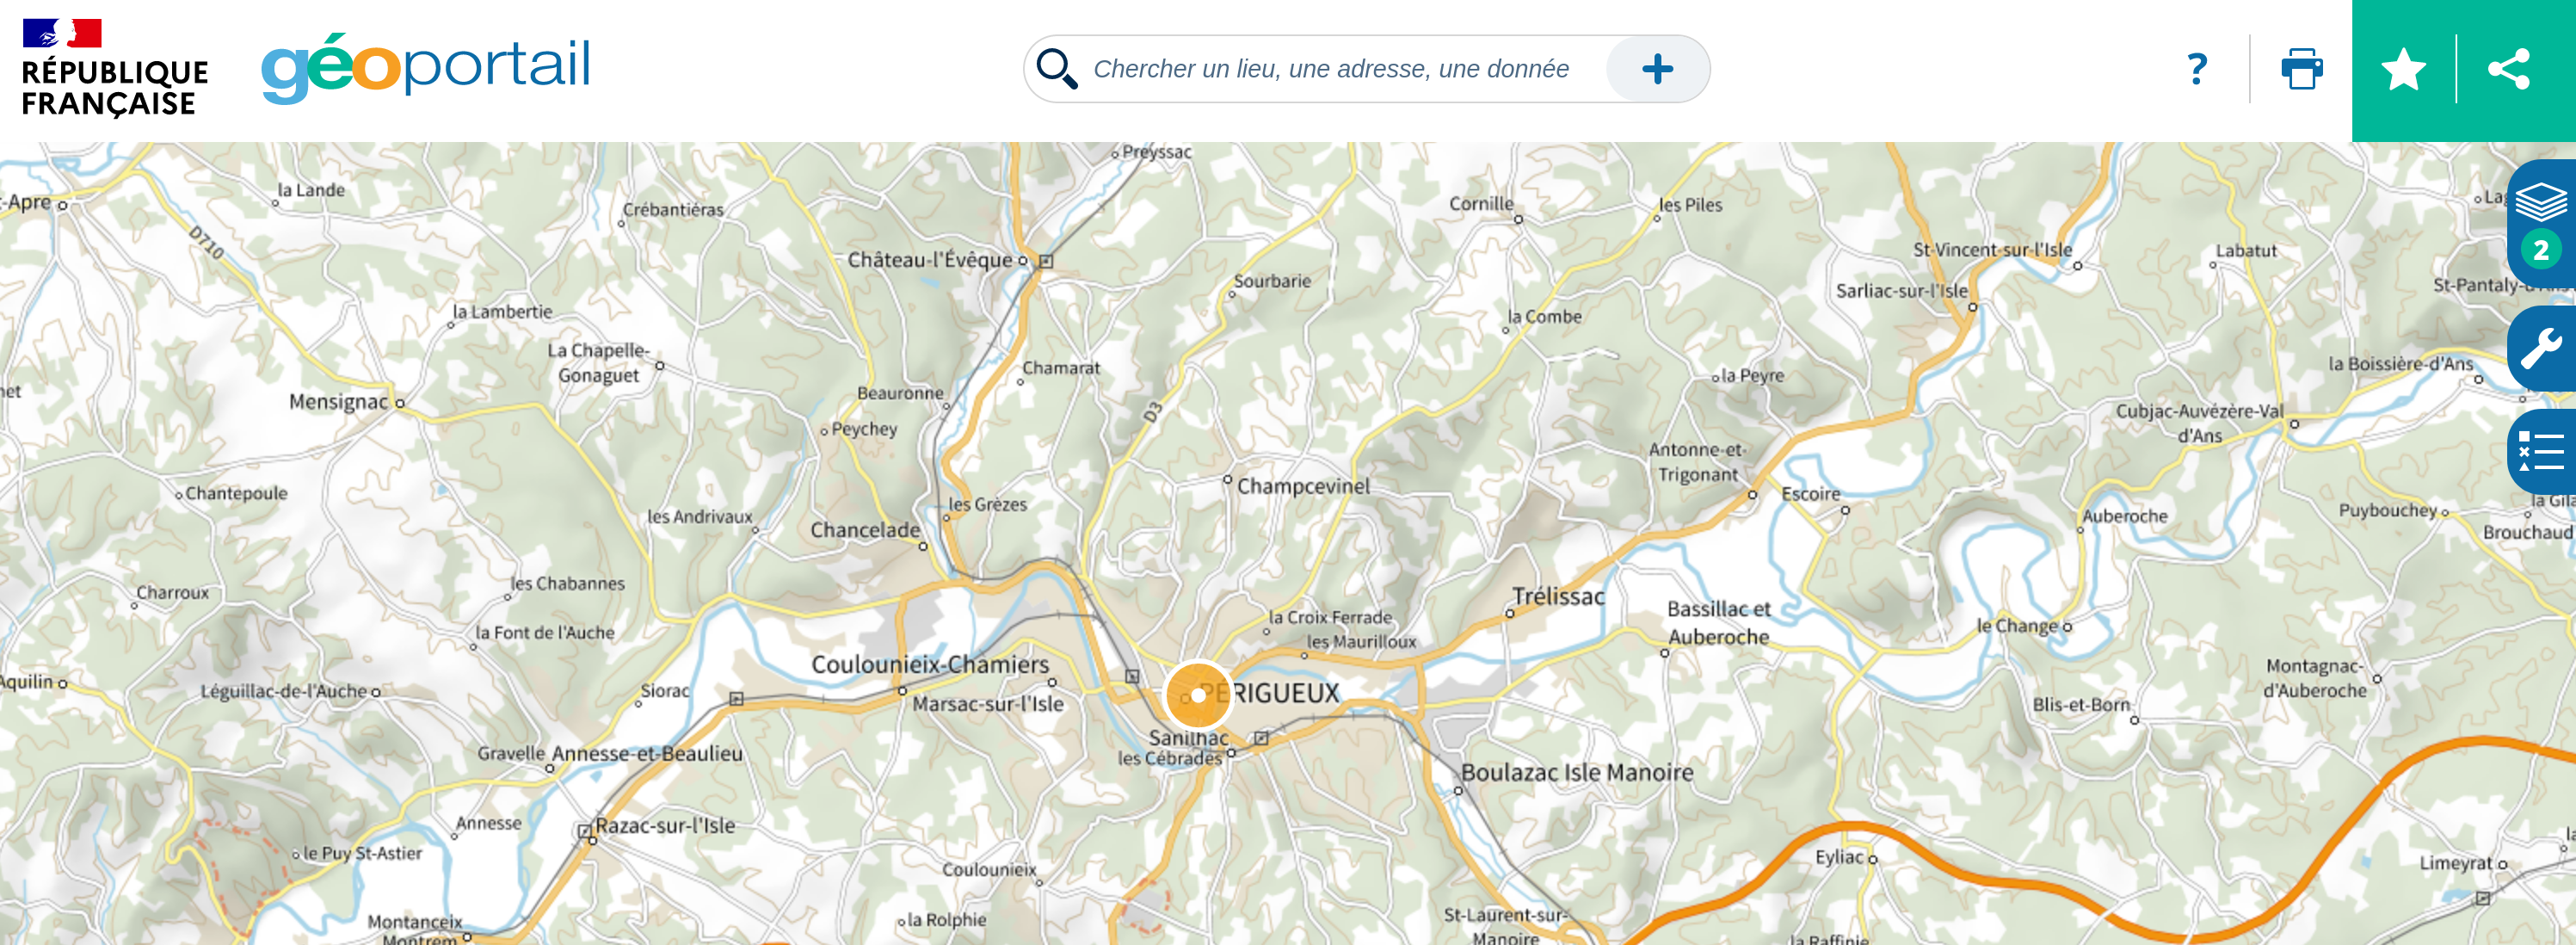
\includegraphics[width=10cm]{ressources/geoportail.png}
    \captionof{figure}{Page Géoportail}
    \label{IMG}
    \end{center}

\end{frame}
\begin{frame}
    \frametitle{}

    \begin{activite}
        \begin{enumerate}
            \item Se rendre sur le site \url{https://www.geoportail.gouv.fr}
            \item Cliquer sur l'icône \emph{Cartes} (figure \ref{gauche})
            \begin{center}
            \centering
            
\includegraphics[width=1cm]{ressources/gauche.png}
            \captionof{figure}{Cartes}
            \label{gauche}
            \end{center}
            \item Choisir le fond \emph{Plan IGN}.
            \item Quelles informations sont disponibles?
            \item Ajouter le fond \emph{Parcelles cadastrales}.
            \item Dispose-t-on des mêmes informations?
        \end{enumerate}
        \end{activite}

\end{frame}
\begin{frame}
    \frametitle{Avant de regarder la correction}
\begin{center}
    \centering
    \includegraphics[width=3cm]{/home/tof/Documents/Cozy/latex-include/stop.png}
    \end{center}
{\Large
    \begin{itemize}
        \item Prendre le temps de réfléchir,
        \item Analyser les messages d'erreur,
        \item Demander au professeur.
    \end{itemize}
}
\end{frame}
\begin{frame}
    \frametitle{Correction}

    Le fond \emph{Plan IGN} fournit de nombreuses informations:
    \begin{itemize}
        \item noms des villes, des lieu-dits\dots
        \item tracés des routes nationales, départementales, autoroutes.
        \item indications sur le relief (zones ombrées).
        \item selon le niveau de zoom, on peut également voir les bâtiments.
    \end{itemize}
Le fond \emph{Parcelles cadastrales} donnent le découpage des propriétés (ou parcelles).

\end{frame}
\begin{frame}
    \frametitle{}

    \begin{activite}
        \begin{enumerate}
            \item Dans le menu \emph{Données thématiques} trouver le fond permettant de faire apparaître les collèges et lycées.
            \item Noter le numéro cadastral de la parcelle du lycée Jay de Beaufort.
            \item À l'aide du menu de droite (figure \ref{droite}) trouver les coordonnées GPS (en degrés sexagésimaux) du bâtiment de l'internat du lycée.
            \begin{center}
            \centering
            
\includegraphics[height=2cm]{ressources/droite.png}
            \captionof{figure}{Outils}
            \label{droite}
            \end{center}
            \item Mesurer la surface de la parcelle du lycée.
        \end{enumerate}
        \end{activite}

\end{frame}
\begin{frame}
    \frametitle{Avant de regarder la correction}
\begin{center}
    \centering
    \includegraphics[width=3cm]{/home/tof/Documents/Cozy/latex-include/stop.png}
    \end{center}
{\Large
    \begin{itemize}
        \item Prendre le temps de réfléchir,
        \item Analyser les messages d'erreur,
        \item Demander au professeur.
    \end{itemize}
}
\end{frame}
\begin{frame}
    \frametitle{Correction}

    Le lycée est sur la parcelle 0338, sur une surface de 16800m². Les coordonnées GPS de l'internat sont:
\begin{itemize}
    \item Latitude: 45,181330°N
    \item Longitude: 0,710249°E
\end{itemize}
Les indications Nord et Est précise la position du lieu par rapport à l'équateur et au méridien de Greenwich (voir cours précédent). Il est à noter que les coordonnées GPS sont très précises: un décalage infime de la souris sur l'écran donne des valeurs légèrement différentes.

\end{frame}
\begin{frame}
    \frametitle{}

    Le professeur a effectué une sortie VTT. Avec sa nouvelle montre il a enregistré sa trace GPS. Il souhaiterait visualiser ses données sur une carte IGN.
    \begin{center}
    \centering
    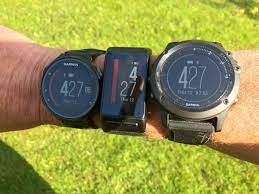
\includegraphics[width=6cm]{ressources/montre.jpeg}
    \end{center}

\end{frame}
\begin{frame}
    \frametitle{}

    
\begin{activite}
\begin{enumerate}
    \item Télécharger et décompresser le fichier \emph{Géoportail - annexe} sur le site \url{https://cviroulaud.github.io}
    \item À l'aide du menu de droite de Géoportail, importer le fichier \emph{trace\_vtt.kml} sur la carte.
    \item Si nécessaire, réorganiser les couches (figure \ref{couche}) pour voir apparaître la trace.
    \begin{center}
    \centering
    
\includegraphics[width=1cm]{ressources/droite-2.png}
    \captionof{figure}{Couches}
    \label{couche}
    \end{center}
    
\end{enumerate}
\end{activite}

\end{frame}
\begin{frame}
    \frametitle{}
\setcounter{compteuractivite}{2}
    \begin{activite}
    \begin{enumerate}
        \setcounter{enumi}{3}
        \item Ajouter le fond de carte \emph{Carte topographique IGN}.
    \item Les traits orange représentent les courbes de niveaux: tous les points sur un même trait sont à la même altitude. Que se passe-t-il quand les traits sont très rapprochés?
    \item Le professeur a-t-il effectué un parcours très accidenté?
    \item Choisir le fond de carte qui permet de visualiser les limites administratives entre les communes.
    \item Sur quelles communes le professeur a-t-il effectué son parcours?
    \end{enumerate}
    \end{activite}

\end{frame}
\begin{frame}
    \frametitle{Avant de regarder la correction}
\begin{center}
    \centering
    \includegraphics[width=3cm]{/home/tof/Documents/Cozy/latex-include/stop.png}
    \end{center}
{\Large
    \begin{itemize}
        \item Prendre le temps de réfléchir,
        \item Analyser les messages d'erreur,
        \item Demander au professeur.
    \end{itemize}
}
\end{frame}
\begin{frame}
    \frametitle{Correction}

    Plus les courbes de niveau sont rapprochées, plus le terrain est pentu. C'est une indication qu'il est important de repérer lors d'une randonnée. Le professeur a roulé sur les communes de Périgueux et Trélissac. Il a longé la commune de Champcevinel.

\end{frame}
\end{document}